\setchapterpreamble[u]{\margintoc}
\chapter{Introduction}
\labch{intro}

\section{Motivation}
Muscle-invasive urothelial bladder cancer (MIBC) happens when the tumour tissue from the bladder starts spreading into the muscle layer of the bladder wall. This event triggers into a more aggressive and potentially life-threatening cancer type. MIBC accounts for approximately 75\% of all bladder cancer cases\cite{Valderrama.BP}. A standard diagnosis is based on the detection of clinical symptoms, imaging studies, cystoscopy, and histopathological examination of biopsy samples to confirm the diagnosis and determine the subtype of tumour\cite{Aragon-Ching}. Treatment approaches for MIBC can come in many forms and usually involve a collaborative effort among surgery, radiation, and medical oncology. Always, the primary goal is to achieve a cure or durable remission while improving the patient’s quality of life. Radical cystectomy (RC), the standard treatment, implies surgical removal of the bladder, surrounding lymph nodes, and sometimes adjacent organs like the prostate or uterus, often supplemented with chemotherapy and radiation therapy\cite{Malkowicz}. Lately, alternative approaches have emerged for patient’s ineligibility for RC due to age or comorbidities. These methods, called neoadjuvant therapies, involve using chemotherapy, immunotherapy or radiation therapy to shrink the tumour before surgical removal. Additionally, immunotherapy, particularly checkpoint inhibitors, has become integral to MIBC treatment, either alone or in combination with traditional therapies to enhance outcomes\cite{Noauthors}. While RC remains the gold standard in the treatment of MIBC, new strategies and treatments using immunotherapy techniques are increasingly improving treatment effectiveness and patient quality of life. In spite of all the advancements, there are still limitations and challenges with current treatments, which move the focus to neoadjuvant approaches.

Based on the administration of therapeutic agents before a main treatment, neoadjuvant chemotherapy (NAC) offers promising results by reducing tumour mass prior to surgery, which enhances the response, and potentially increases the likelihood of successful outcomes. Neoadjuvant approaches show a good synergy with immunotherapy. By combining both techniques, we can improve treatment efficacy, and patient prognosis. Furthermore, neoadjuvant strategies mitigate the morbidity associated with RC, enabling less invasive surgical procedures and better post-operative recovery. On top of that, neoadjuvant approaches enable personalised medicine, tailoring treatments based on individual patient characteristics and optimal outcomes. Reducing the need for radical surgeries and enhancing treatment responses, thanks to neoadjuvant approaches we can contribute to improved quality of life for MIBC patients \cite{7}\cite{Nair}.

Retrospective analyses in several tumour types, including urothelial bladder cancer, have identified gene expression profiles as predictive biomarkers of response to Immune Checkpoint Inhibitor (ICI)\sidenote{Immune checkpoints are specific proteins on the surface of immune cells that act as natural brakes to prevent the immune system from being overactive and attacking the body's own healthy tissues. \textbf{Immune checkpoint inhibitors} are a type of immunotherapy that blocks specifically these proteins.}. In these studies, the tumour inflammation score (TIS) is one of the most robust biomarkers predictive of response to ICI, and its ability to discriminate is preserved across tumour types. The TIS has also been associated at the PanCancer level with prognosis and has been proposed as an indirect measure of an inflamed tumour phenotype that might guide immunotherapy across cancer types\cite{Danaher2018} \cite{Damotte2019}. However, a major problem in translational research is that few of the promising markers identified in retrospective studies, including the TIS, are applied prospectively to demonstrate clinical utility to stratify and optimize patient treatment.

The DUTRENEO clinical trial\cite{DUTRENEO} was uniquely designed to prospectively test the usefulness of stratifying patients with MIBC based on the TIS to select patients who could benefit more from neoadjuvant ICI, and to compare this arm to conventional NAC. This phase II clinical trial represents a significant advancement in the exploration of neoadjuvant approaches together with immunotherapy for managing MIBC and an opportunity to research the intrinsic mechanisms separating the immune infiltration nature of tumours. The underlying hypothesis posited that the expression of certain genes within this signature could predict a favourable response to immunotherapy treatment. To test this hypothesis, the study evaluated a combination of durvalumab and tremelimumab, two drugs that belong to the monoclonal antibody group, have shown promising results for the treatment of various cancers, including MIBC. Durvalumab, an anti-programmed cell death ligand-1 (PD-L1) antibody, operates by obstructing the PD-L1 and PD-1 interaction, thereby reinforcing the immune system’s response against cancer cells. On the other hand, tremelimumab, an anti-cytotoxic T lymphocyte-associated antigen 4 (CTLA-4) antibody, impedes the activity of regulatory T cells that dampen the immune response. This trial targeted a subset of MIBC patients identified through a tumour pro-inflammatory IFNgamma signature, quantified as the tumour inflammation score (TIS). The results of DUTRENEO clinical trial unveiled a notable achievement, with the combination of durvalumab and tremelimumab yielding a complete pathological response rate of 34.8\%, coupled with a favourable safety profile. Intriguingly, however, the correlation between the TIS and treatment response within this group appeared less evident. These findings advocate for continued exploration of immunotherapeutic interventions in the neoadjuvant setting, alongside endeavours to elucidate biomarkers capable of predicting treatment response. 

Consequently, further research from multiple points of view is indispensable to determining the optimal use of this combination and comprehending its shaded benefits and limitations within distinct patient populations. Since bulk transcriptomic approaches have shown limited success in identifying biomarkers capable of reliably stratifying patients and guiding optimal treatment selection, alternative technologies must be investigated. That is where technologies such as spatial transcriptomics (ST) may provide valuable insights into the tumour microenvironment and improve our understanding of the mechanisms underlying treatment response.

\section{What is spatial transcriptomics}
\labsec{ST_intro}

Gene expression is the process by which the information encoded in a gene is turned into a function. This mostly occurs via the transcription of RNA molecules that code for proteins or non-coding RNA molecules that serve other functions\cite{NHGRI}. Whereas genomics studies an organism’s genome or the entire DNA sequence, transcriptomics studies all RNA transcripts that are being produced under a certain condition. The entire collection of mRNA sequences in a cell, or the transcriptome, allows scientists and researchers to determine when and where genes are turned on and off in an organism\cite{Dr.Cartwright}. ST is a newly emerging field that enables high-throughput investigation of the spatial localization of transcripts and related analyses in various applications for biological systems. By transitioning from conventional biological studies to “in situ” biology, ST can provide transcriptome-scale spatial information\cite{Han-Eol.Park} . 

ST has emerged as a transformative approach in biology by enabling the measurement of gene expression directly within intact tissue, thereby preserving the spatial context that is lost in conventional bulk and single-cell RNA sequencing (scRNA-seq)\cite{Cameron.G.W}. This spatial information is biologically critical because cellular identity and function are not only determined by intrinsic gene expression programs but also by the local microenvironment, including cell–cell interactions, signaling gradients, and tissue architecture \cite{Han-Eol.Park}. In this sense, spatial tachnologies allows us to move from the cellular level of study to the tissue level. As a result, ST makes it possible to investigate how cells organize into functional niches, how developmental processes are coordinated, and how diseases such as cancer emerge as structured ecosystems rather than homogeneous masses. For example, spatial approaches have revealed that tumor cell states and immune environments are segregated into distinct niches and that interactions between cancer cells and surrounding stromal or immune cells are spatially organized and functionally relevant \cite{Mengyi.Liu}. Imaging-based platforms such as Xenium build on these principles by enabling highly multiplexed, single-cell to subcellular resolution detection of hundreds to thousands of transcripts in situ, allowing precise mapping of cell types, states, and their physical interactions within tissue architecture \cite{Hyun.Ju.Lim}. This makes Xenium particularly powerful for dissecting complex biological systems such as tumor–immune interfaces or developmental gradients. However, in pharmaceutical contexts, limitations remain, including constrained gene panels compared to whole-transcriptome approaches, challenges in scaling throughput, and the need for careful experimental design to capture clinically relevant biology. Despite these constraints, Xenium holds significant potential for drug development by enabling the identification of spatial biomarkers, uncovering mechanisms of response and resistance, and refining patient stratification through direct observation of cellular interactions within their native tissue context, ultimately bridging molecular insights with tissue-level biology.

\section{Existing technologies}
\labsec{VisiumVSXenium}
Messenger RNA (mRNA) transcripts are single-stranded RNA molecules that carry genetic instructions from DNA to the ribosomes. Measuring mRNA provides a way of estimating which genes are active within a cell. ST technologies, such as Visium and Xenium, are designed to measure gene expression directly within tissue while preserving spatial information. In other words, they allow the identification of which genes are being expressed and where those RNA molecules are physically located within the tissue. To further explain what ST is and why the analysis of this type of data is highly complex, it is useful to consider the evolution of transcriptomic technologies.

Initially, bulk RNA sequencing was performed using tissue samples in which transcripts were extracted from all cells simultaneously, allowing only the estimation of average gene expression across the sample. Subsequently, single-cell technologies emerged, enabling the reading of transcripts from each individual cell within the sample, thereby making it possible to determine the expression level of each gene in every cell. Finally, ST technologies emerged, enabling not only the identification of genes in single cells or groups of cells but also the determination of where those cells are physically located within the tissue. \reffig{B_SC_ST} shows a graphical representation of each of the aforementioned technologies.

\begin{figure}[H]
\centering
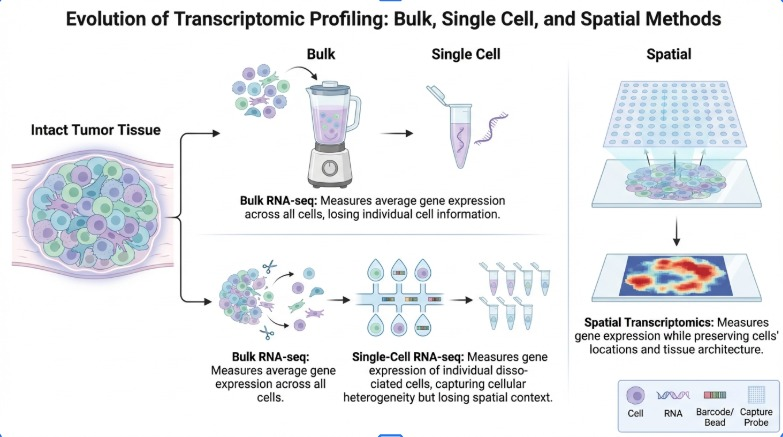
\includegraphics[width=\textwidth]{images/Bulk_SingleCell_Spatial.jpeg}
\caption{Evolution of Transcriptomic Profiling (figure made with Figure Labs).}
\labfig{B_SC_ST}
\end{figure}

ST technologies emerged in 2019, when two major platforms entered the market, one of them being Visium. Visium divided the tissue into a grid of discrete barcoded capture spots, where several cells could be read within each spot, enabling the detection of mRNA transcripts while preserving structural information. However, the technology still presented several limitations. Since transcripts could not be assigned to individual cells, analyses still relied on averages and median values rather than true single-cell measurements. Additionally, information loss occurred between spots, as the physical gaps between them left regions of tissue unread. These limitations motivated the emergence of Xenium in 2022, a technology capable of reading transcripts at subcellular resolution. Xenium did not require the tissue to be physically divided, thereby preserving the entire tissue architecture and retaining all structural information.

However, for every new axis of information gained, another was lost. In a typical scRNA-seq experiment, between $\sim1,000$ and $\sim11,000$ unique genes can be detected per cell \cite{Victoria.Probst}, depending on the technology and cell type. In contrast, ST technologies generally detect only hundreds of genes per measurement, although some platforms are now capable of profiling thousands. These technologies are evolving rapidly, with whole-genome, transcriptome, and even proteome-scale spatial profiling becoming increasingly feasible \cite{Tsai-Ying.Chen}. This Master's thesis was conducted using Xenium technology with a multi-tissue panel of only 377 genes.

The number of genes detected per cell can facilitate intermediate analysis steps, such as cell type annotation. In general, the greater the number of detected genes per cell, the higher the ability to distinguish between different cell populations. However, this limitation is common across all transcriptomics technologies and depends not only on the technology itself, but also on the number and quality of transcripts captured in the experiment. Therefore, cell type annotation is influenced not only by the number of detected genes, but also by transcript abundance and data quality. A broader variety of detected genes does not necessarily guarantee easier or more accurate annotation.

As shown in \reffig{Figure12}, the Xenium MIBC dataset (A) presents a much more diffuse and overlapping clustering structure compared with the scRNA-seq dataset (B), where clusters are more clearly separated and easier to identify. The reduced number of genes detected per cell in Xenium limits transcriptional resolution and complicates the discrimination between closely related cell populations. Nevertheless, despite this lower resolution, the principal biological structures and major cellular populations remain detectable.

\begin{figure}[H]
\centering

\includegraphics[width=\textwidth]{images/STvsSC_Clustering.png}
\caption{Example illustrating how the number of unique genes complicates the analysis with a UMAP\textsuperscript{a}. Figure A corresponds to the dataset used in this thesis, generated using a ST technology with only 377 unique genes. Figure B was extracted from \href{https://medium.com/@mohamed.y.elsadec_56085/a-comparative-analysis-of-clustering-scrna-seq-data-using-pca-based-and-gnn-driven-approaches-24c9fb8d5ec8}{this blog} and corresponds to a single-cell technology dataset. }
\labfig{Figure12}
\end{figure}
\footnotesize{\textsuperscript{a}A UMAP (Uniform Manifold Approximation and Projection) is a dimensionality reduction technique that projects high-dimensional data, such as gene expression profiles, into a two-dimensional space, allowing similar cells to cluster together while preserving their underlying biological relationships.}

This effect can also be observed in the annotated MIBC datasets shown in \reffig{figure3}. In the Xenium dataset (A), the same dataset used in \reffig{Figure12}, cell populations display substantial overlap, making the assignment of precise labels more challenging, particularly for immune-related subtypes. In contrast, the MIBC single-cell dataset (B) exhibits well-defined and compact clusters that facilitate the identification of epithelial cells, fibroblasts, endothelial cells, granulocytes, T cells, B cells, and other immune populations. These key differences illustrate that the difficulty in annotation is largely driven by the quality and quantity of transcriptomic information available per cell rather than by the spatial technology itself.

\begin{figure}[H]
\centering

\includegraphics[width=\textwidth]{images/STvsSC_MIBC.png}
\caption{Comparison of cell type annotation in muscle-invasive bladder cancer (MIBC) using spatial versus single-cell transcriptomics. \textbf{(A)} UMAP projection of Xenium ST data (377 genes) used in this thesis, with cell types annotated using SingleR. Cluster boundaries are diffuse and several populations overlap, reflecting the limited gene panel. \textbf{(B)} UMAP projection of single-cell RNA-seq data from MIBC (>3{,}000 genes) used in \cite{Dongxu.Qiu}, with cell types annotated using simple clustering, showing well-separated clusters with clearly resolved immune subpopulations (M1, M2, dendritic cells, Tregs, CD4\textsuperscript{+}/CD8\textsuperscript{+} T cells). The contrast illustrates how a reduced gene panel hampers fine-grained cell type discrimination, particularly within the immune compartment.}
\labfig{figure3}
\end{figure}

ST technologies are relatively recent, as a consequence:

\begin{itemize}
\item there are still few standardized pipelines specifically designed for Xenium and Visium,
\item the available literature remains limited, particularly regarding MIBC,
\item many computational methods remain experimental and have barely demonstrated superior performance compared with currently used basic statistical methods,
\item best practices are still evolving.
\end{itemize}

\section{Main Differences Between Visium and Xenium}

ST technologies such as Visium and Xenium are designed to measure gene expression directly within tissue while preserving spatial information. In other words, they make it possible to determine not only which genes are being expressed, but also where those transcripts are physically located within the tissue architecture. Both technologies analyze mRNA molecules, which are temporary copies of genes used by cells to synthesize proteins. Although Visium and Xenium pursue the same biological objective, they differ substantially in their methodology, spatial resolution, and analytical capabilities.

Visium is a spot-based\sidenote{Spots in 10x Genomics Visium are specific, spatially barcoded capture locations on a tissue section array.} ST technology in which tissue sections are placed onto specialized capture slides containing thousands of spatially indexed spots. Each spot contains DNA oligonucleotides\sidenote{DNA oligonucleotides (often called ``oligos'') are short, single-stranded segments of synthetic DNA, typically ranging from 10 to 50 nucleotides in length.} composed of a poly(dT) sequence\sidenote{A poly(dT) sequence is a short, single-stranded stretch of DNA consisting entirely of repeating thymine (T) nucleotides.}, a spatial barcode, and a unique molecular identifier (UMI)\sidenote{A Unique Molecular Identifier (UMI) is a short, random nucleotide sequence attached to individual DNA or RNA molecules before they are amplified and sequenced.}. The poly(dT) sequence captures mRNA molecules through their poly(A) tails after the tissue is permeabilized and RNA diffuses out of the cells. Because each spot captures transcripts originating from multiple nearby cells, the resulting data generally lacks true single-cell resolution. After RNA capture, the molecules are reverse transcribed into complementary DNA (cDNA)\sidenote{Complementary DNA (cDNA) is synthetic DNA created by transcribing a specific mRNA template using an enzyme called reverse transcriptase.}, which preserves both the gene identity and the spatial barcode information. The cDNA is subsequently amplified using PCR\sidenote{PCR stands for Polymerase Chain Reaction. It is a laboratory technique used to make millions or billions of copies of a specific DNA segment, acting as ``molecular photocopying.''} and prepared into sequencing libraries for next-generation sequencing (NGS)\sidenote{Next-generation sequencing (NGS) is a massively parallel DNA and RNA sequencing technology}. Sequencing reads\sidenote{Sequencing reads are the fundamental data output of DNA and RNA sequencing. They are short strings of letters (A, T, C, G) representing the exact sequence of nucleotide bases from a single fragment of genetic material. Essentially, they are the individual puzzle pieces used to reconstruct a full genome.} are then mapped back to genes and spatial locations, ultimately generating a gene-by-spot expression matrix that represents the transcriptional landscape of the tissue.

In contrast, Xenium is an imaging-based ST technology capable of achieving single-cell and subcellular resolution. Rather than sequencing RNA captured from spatial spots, Xenium directly visualizes RNA molecules inside intact tissue sections. Unlike Visium, Xenium relies on predefined targeted gene panels, which may include hundreds or thousands of selected genes chosen according to biological hypotheses, signaling pathways\sidenote{Describes a series of chemical reactions in which a group of molecules in a cell work together to control a cell function, such as cell division or cell death.}, or prior scRNA-seq references. For each gene, multiple DNA probes\sidenote{DNA probes are short, single-stranded segments of DNA designed to detect a specific, complementary sequence of genetic material.} are designed to hybridize specifically to the target RNA molecules within the tissue. These probes bind directly to transcripts in situ, preserving the precise spatial localization of each molecule without requiring RNA diffusion\sidenote{RNA diffusion refers to the movement of RNA molecules through the cell's cytoplasm to specific locations}.

Following probe hybridization\sidenote{Probe hybridization is a molecular biology technique where a short, labeled fragment of DNA or RNA (the ``probe'') binds to a specific, complementary target sequence within a complex DNA or RNA sample.}, signal amplification is performed through rolling circle amplification (RCA)\sidenote{Rolling circle amplification (RCA) is an isothermal (constant-temperature) enzymatic process that uses a small circular DNA template to create a long, single-stranded DNA molecule.}, generating fluorescent signals strong enough to be detected microscopically. The tissue is then imaged through multiple fluorescence cycles, during which different genes generate characteristic fluorescent patterns. Computational decoding algorithms interpret these fluorescence signatures and assign each detected signal to its corresponding gene identity through predefined barcode patterns. This process enables the reconstruction of transcript locations with subcellular precision and provides highly detailed spatial maps of gene expression.

An additional fundamental component of Xenium analysis is cell segmentation, which determines which transcripts belong to each individual cell. Tissue sections are stained using nuclear markers such as DAPI\sidenote{DAPI (4$'$,6-diamidino-2-phenylindole) is a popular fluorescent stain used in cell biology and microscopy to visualize DNA.} and, when available, membrane markers that facilitate the identification of cellular boundaries. Image analysis algorithms detect nuclei and estimate cell contours, after which segmentation methods computationally define individual cellular compartments. Detected transcripts are subsequently assigned to cells according to their spatial coordinates relative to the segmented boundaries. The final output therefore includes both a gene-by-cell expression matrix and the exact spatial coordinates of every detected transcript, enabling downstream analyses focused on cellular organization, tissue architecture, and cell-cell interactions.

\begin{center}
\begin{minipage}{\textwidth}
\centering
\small

\begin{tabular}{|p{0.23\textwidth}|p{0.23\textwidth}|p{0.34\textwidth}|}
\hline
\textbf{Feature} & \textbf{Visium} & \textbf{Xenium} \\
\hline
Resolution & Spot-level & Single-cell/subcellular \\
\hline
Detection method & Sequencing & Imaging \\
\hline
Transcript location & Spot coordinates & Cell coordinates \\
\hline
Coverage & Whole transcriptome & Targeted panel\textsuperscript{b} \\
\hline
Main output & Gene-by-spot matrix & Gene-by-cell matrix and transcript coordinates \\
\hline
\end{tabular}

\vspace{0.5em}

\captionof{table}[Visium vs. Xenium]{Main differences between Visium and Xenium technologies.}

\vspace{0.3em}

\raggedright
\footnotesize
\textsuperscript{b} Some newer Xenium-related technologies may support broader transcriptome profiling, but standard Xenium workflows are generally targeted-panel based.

\end{minipage}
\end{center}

\section{The Main Idea}

This Master's thesis was carried out in the Cancer Immunogenomics Laboratory, led by Eduard Porta, at the Josep Carreras Leukaemia Research Institute. The laboratory participated in the development of the DUTRENEO clinical trial\cite{Grande.et.al}. DUTRENEO was a multicentre, open-label, phase II study conducted across 11 Spanish tertiary care hospitals \cite{Grande.et.al}. The trial investigated whether an 18-gene TIS\sidenote{The Tumour Inflammation Signature (TIS) is a validated 18-gene expression profile that measures a pre-existing but suppressed adaptive immune response within the tumour microenvironment. It identifies ``hot'' (inflamed) tumours that are more likely to respond to immune checkpoint inhibitors (ICI).} could robustly identify patients likely to respond to ICI across multiple tumour types, and whether it could therefore be used to stratify patients with localised muscle-invasive bladder cancer (MIBC) to receive either neoadjuvant ICI (durvalumab + tremelimumab) or standard cisplatin-based NAC. Patients with a high TIS score tumour (immune-hot) were randomized to receive an ICI combination consisting of durvalumab and tremelimumab (ICI) or standard cisplatin-based NAC, according to the physician's choice. To acquire a better understanding of the value of the signature, they also included patients whose tumours had a low TIS score (immune-cold) and who were treated with standard cisplatin-based NAC. 

Unfortunately, the clinical trial did not achieve the expected results, as the TIS alone was not sufficient to reliably stratify MIBC patients according to the treatment from which they were most likely to benefit. To further investigate the biological mechanisms underlying this outcome, a ST layer was incorporated with the aim of providing additional insight into the tumour microenvironment and treatment response.

To characterise the samples more comprehensively and improve the prediction of therapeutic response, multiple molecular platforms were employed, providing both whole-transcriptome coverage and single-cell resolution:

\begin{itemize}
	\item \textbf{Formalin-fixed paraffin-embedded (FFPE) tissues} obtained during the TURBT were used for whole-exome sequencing (WES) ($n = 44$)
	\item \textbf{Bulk RNA sequencing} was performed on $n = 57$ samples.
    \item \textbf{Spatial transcriptomics} was carried out using both Visium ($n = 33$) and Xenium ($n = 20$).
\end{itemize}

The Visium dataset comprised 99,028 spots across all samples, with an average of 4,097 unique genes detected per spot. In contrast, the Xenium dataset included the analysis of 377 genes in 5,399,355 cells, with a median of 48 transcripts and 28 genes detected per cell.\sidenote{The differences between Visium and Xenium and what they are are explained in the section \vrefsec{VisiumVSXenium} }

This research group specialises in ST\sidenote{A more detailed explanation of this technology is provided in the next section, \vrefch{ST_intro}.}. The contribution of this thesis to the broader project was to perform a basic transcriptomic analysis of post-treatment samples. Analysing the local microenvironment of tumour cells can provide important insights into their complex interactions with surrounding cell populations, including immune cells. By quantifying the abundance and spatial proximity of specific immune cell types in the vicinity of tumour cells through neighbourhood analysis, patterns may emerge that reveal relevant associations between cellular populations. Such analyses can uncover key aspects of tumour--immune dynamics and may ultimately inform therapeutic strategies. This method enables an in-depth exploration of spatial interactions among different cell types, which is crucial for research in oncology, immunology, and developmental biology \cite{Aryeh.Silver}.

Following a brief introduction to this profiling technology and its potential, the history of transcriptomic profiling will be reviewed, together with a discussion of how these approaches differ from ST, both positively and negatively. Subsequently, all steps of the analysis performed in this thesis will be described, from the review of the state of the art, Quality Control (QC)\vrefch{QC} , and cell annotation \vrefch{cellAnn} to neighbourhood analysis \vrefch{NA} and its biological conclusions\vrefch{Con}.

\section{Objectives}

The main objective of this work was to gain a deeper understanding of ST technologies and to develop the necessary expertise to properly analyze this type of data. To achieve this, an initial review of state-of-the-art methodologies and current analytical practices in the field was conducted in order to identify robust and reproducible approaches for ST data analysis. This assessment provided the basis for investigating and implementing the different analytical steps required in ST workflows. 

Subsequently, a complete introductory workflow was established for both Xenium and Visium datasets, covering the main preprocessing and analytical procedures commonly used in ST studies, including QC, data normalization, dimensionality reduction, clustering, and cell type annotation. Based on the knowledge acquired during this process, the analytical procedures used within the host laboratory were further standardized into a more consistent and unified workflow, reducing variability arising from individually developed analysis strategies. Special attention was given to understanding the challenges associated with lower gene detection per cell and how this affects downstream analyses and biological interpretation.

Beyond the basic workflow, the project focused on further exploring Xenium data in order to better understand the biological information that can be extracted from spatially resolved transcriptomic experiments. In particular, a neighbourhood analysis was performed to study spatial relationships between different cell populations and investigate how cells interact within the tumor microenvironment of muscle-invasive bladder cancer (MIBC). This additional analysis provided practical experience in interpreting spatial organization patterns and translating computational results into biologically meaningful conclusions. 

Finally, neighbourhood and spatial interaction analyses were performed to explore cellular relationships within the tumour microenvironment and to identify spatial features that could explain the discordance between TIS classification and clinical response observed in the DUTRENEO trial. Through this approach, the study aimed to determine whether spatially resolved patterns of  cellular organization provide additional biological information beyond conventional bulk transcriptomic biomarkers, thereby contributing to a better understanding of response mechanisms to neoadjuvant immunotherapy in MIBC.



% %%%%%%%%%%%%%%%%%%%%%%%%%%%%%%%%%%%%%%%%%%%%%%%%%%%%%%%%%%%%%%%%%%%%%%%%%%%%%%%%%%%%%%%%%%%%%%%%%%%%%
% \section{What This Class Does}
% \labsec{does}

% The main features are the following:

% \begin{description}
% 	\item[Page Layout] The text width is reduced to improve readability 
% 	and make space for the margins, where any sort of elements can be 
% 	displayed.
% 	\item[Chapter Headings] As opposed to Tufte-Latex, we provide a 
% 	variety of chapter headings among which to choose; examples will be 
% 	seen in later chapters.
% 	\item[Page Headers] They span the whole page, margins included, and, 
% 	in twoside mode, display alternatively the chapter and the section 
% 	name.\sidenote[][-2mm]{This is another departure from Tufte's 
% 	design.}
% 	\item[Matters] The commands \Command{frontmatter}, 
% 	\Command{mainmatter} and \Command{backmatter} have been redefined in 
% 	order to have automatically wide margins in the main matter, and 
% 	narrow margins in the front and back matters. However, the page 
% 	style can be changed at any moment, even in the middle of the 
% 	document.
% 	\item[Margin text] We provide commands \Command{sidenote} and 
% 	\Command{marginnote} to put text in the 
% 	margins.\sidenote[][-2mm]{Sidenotes (like this!) are numbered while 
% 	marginnotes are not}
% 	\item[Margin figs/tabs] A couple of useful environments is 
% 	\Environment{marginfigure} and \Environment{margintable}, which, not 
% 	surprisingly, allow you to put figures and tables in the margins 
% 	(\cfr \reffig{marginmonalisa}). 
% 	\item[Margin toc] Finally, since we have wide margins, why don't add 
% 	a little table of contents in them? See \Command{margintoc} for 
% 	that.
% 	\item[Hyperref] \Package{hyperref} is loaded and by default we try 
% 	to add bookmarks in a sensible way; in particular, the bookmarks 
% 	levels are automatically reset at \Command{appendix} and 
% 	\Command{backmatter}. Moreover, we also provide a small package to 
% 	ease the hyperreferencing of other parts of the text.
% 	\item[Bibliography] We want the reader to be able to know what has 
% 	been cited without having to go to the end of the document every 
% 	time, so citations go in the margins as well as at the end, as in 
% 	Tufte-Latex. Unlike that class, however, you are free to customise 
% 	the citations as you wish.
% \end{description}

% \begin{marginfigure}[-5.5cm]
% 	\includegraphics{monalisa}
% 	\caption[The Mona Lisa]{The Mona Lisa.\\ 
% 	\url{https://commons.wikimedia.org/wiki/File:Mona_Lisa,_by_Leonardo_da_Vinci,_from_C2RMF_retouched.jpg}}
% 	\labfig{marginmonalisa}
% \end{marginfigure}

% The order of the title pages, table of contents and preface can be 
% easily changed, as in any \LaTeX\ document. In addition, the class is 
% based on \KOMAScript's \Class{scrbook}, therefore it inherits all the 
% goodies of that.

% \section{What This Class Does Not Do}
% \labsec{doesnot}

% As anticipated, further customisation of the book is left to the user. 
% Indeed, every book may have sidenotes, margin figures and so on, but 
% each book will have its own fonts, toc style, special environments and 
% so on. For this reason, in addition to the class, we provide only 
% sensible defaults, but if these features are not needed, they can be 
% left out. These special packages are located in the \Path{style} 
% directory, which is organised as follows:

% \begin{description}
% 	\item[kao.sty] This package contains the most important definitions 
% 	of macros and specifications of page layout. It is the heart of the 
% 	\Class{kaobook}.
% 	\item[kaobiblio.sty] Contains commands to add citations and 
% 	customise the bibliography.
% 	\item[packages.sty] Loads additional packages to decorate the 
% 	writing with special contents (for instance, the \Package{listing} 
% 	package is loaded here as it is not required in every book). There 
% 	are also defined some useful commands to print the same words always 
% 	in the same way, \eg latin words in italics or \Package{packages} in 
% 	verbatim.
% 	\item[kaorefs.sty] Some useful commands to manage labeling and 
% 	referencing, again to ensure that the same elements are referenced 
% 	always in a consistent way.
% 	\item[environments.sty] Provides special environments, like boxes. 
% 	Both simple and complex environments are available; by complex we 
% 	mean that they are endowed with a counter, floating and can be put 
% 	in a special table of contents.\sidenote[][-2mm]{See 
% 	\vrefch{mathematics} for some examples.}
% 	\item[theorems.sty] The style of mathematical environments. 
% 	Actually, there are two such packages: one is for plain theorems,
% 	\ie the theorems are printed in plain text; the other uses 
% 	\Package{mdframed} to draw a box around theorems. You can plug the 
% 	most appropriate style into its document.
% \end{description}

% \marginnote[2mm]{The audacious users might feel tempted to edit some of 
% these packages. I'd be immensely happy if they sent me examples of what 
% they have been able to do!}

% In the rest of the book, I shall assume that the reader is not a novice 
% in the use of \LaTeX, and refer to the documentation of the packages 
% used in this class for things that are already explained there. 
% Moreover, I assume that the reader is willing to make minor edits to the 
% provided packages for styles, environments and commands, if he or she 
% does not like the default settings.

% \section{How to Use This Class}

% Either if you are using the template from 
% \href{http://latextemplates.org/template/kaobook}{latextemplates}, or if 
% you cloned the GitHub 
% \href{https://www.github.com/fmarotta/kaobook}{repository}, there are 
% infinite ways to use the \Class{kaobook} class in practice, but we will 
% discuss only two of them. The first is to find the \Path{main.tex} file 
% which I used to write this book, and edit it; this will probably involve 
% a lot of text-deleting, copying-and-pasting, and rewriting. The second 
% way is to start almost from scratch and use the \Path{skeleton.tex} 
% file, which is a cleaned-up version of the \Path{main.tex}; even if you 
% choose the second way, you may find it useful to draw inspiration from 
% the \Path{main.tex} file.

% To compile the document, assuming that its name is \Path{main.tex}, you 
% will have to run the following sequence of commands:

% \begin{lstlisting}[style=kaolstplain,linewidth=1.5\textwidth]
% pdflatex main # Compile template
% makeindex main.nlo -s nomencl.ist -o main.nls # Compile nomenclature
% makeindex main # Compile index
% biber main # Compile bibliography
% makeglossaries main # Compile glossary
% pdflatex main # Compile template again
% pdflatex main # Compile template again
% \end{lstlisting}

% You may need to compile the template some more times in order for some 
% errors to disappear. For any support requests, please ask a question on 
% \url{tex.stackexchange.org} with the tag \enquote{kaobook}, open an 
% issue on GitHub, or contact the author via e-mail.
